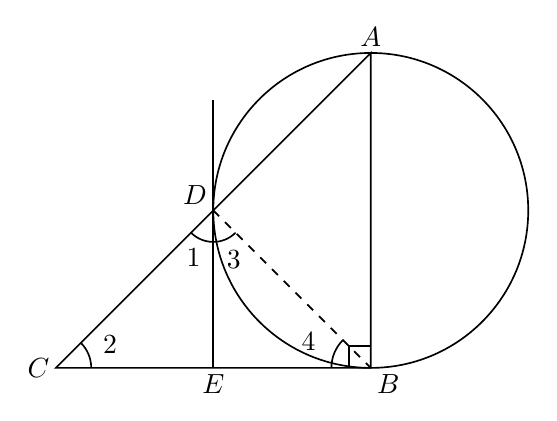
\begin{tikzpicture}[x=1cm,y=1cm,line width=.6pt,font=\normalsize]
\usetikzlibrary{angles,quotes}
\coordinate (A) at (0.0000,4.0000);
\coordinate (B) at (0.0000,0.0000);
\coordinate (C) at (-4.0000,0.0000);
\coordinate (O) at (0.0000,2.0000);
\coordinate (D) at (-2.0000,2.0000);
\coordinate (E) at (-2.0000,0.0000);
\coordinate (T) at (-2.0000,3.4000);
\draw (O) circle[radius=2cm];
\draw (A)--(B)--(C)--cycle;
\draw (E)--(T);
\draw[dashed] (D)--(B);
\draw (-0.2800,0.0000)--(-0.2800,0.2800)--(0.0000,0.2800);
\draw (D) ++(225:0.4000cm) arc[start angle=225,end angle=270,radius=0.4000cm];
\draw (C) ++(0:0.4500cm) arc[start angle=0,end angle=45,radius=0.4500cm];
\draw (D) ++(270:0.4000cm) arc[start angle=270,end angle=315,radius=0.4000cm];
\draw (B) ++(135:0.5000cm) arc[start angle=135,end angle=180,radius=0.5000cm];
\node[above=2pt,inner sep=0pt] at (A) {$A$};
\node[below right=2pt,inner sep=0pt] at (B) {$B$};
\node[left=2pt,inner sep=0pt] at (C) {$C$};
\node[above left=2pt,inner sep=0pt] at (D) {$D$};
\node[below=2pt,inner sep=0pt] at (E) {$E$};
\node at (-2.2500,1.4000) {$1$};
\node at (-3.3100,0.2900) {$2$};
\node at (-1.7400,1.3700) {$3$};
\node at (-0.7900,0.3300) {$4$};
\end{tikzpicture}
